\section{Adquisición de conocimientos}
Para poder enfrentarnos con garantías al desarrollo del proyecto fue necesario
adquirir una \textbf{base de conocimientos} que nos permitiera entender los
conceptos que se iban a usar y las herramientas para trabajar con ellos. Así,
fuimos guiándonos por la intuición y, sobre todo, por las necesidades que iban
surgiendo. 

Los conceptos que se presentan a continuación son básicos para comprender cómo
funciona el módulo de análisis del proyecto.

\subsection{El sonido}
Un \textbf{sonido} es una vibración que se propaga por un medio
elástico en forma de onda. Estas vibraciones se transmiten de forma
longitudinal, esto es, en la misma dirección en la que se propaga la
onda. El medio más común para la transmisión del sonido es el
\textbf{aire}. 

El sonido, en su forma más simple, se compone de una sola onda
sinusoidal básica, con las características tradicionales: amplitud,
frecuencia y fase. Una \textbf{onda sinusoidal} es aquella cuyos
valores se calculan utilizando funciones seno.

\subsubsection{Frecuencia y tono}
La \textbf{frecuencia} mide el número de oscilaciones de la onda por
unidad de tiempo. Por regla general, se utiliza el \textbf{hercio}
como unidad de medida de frecuencia, que indica la cantidad de
repeticiones por segundo. La frecuencia determinará la \textbf{altura}
del sonido, es decir, cómo de grave o agudo es. Los sonidos graves
tienen una frecuencia baja, mientras que los sonidos agudos tienen una
frecuencia alta.

A lo largo de los años se ha establecido un estándar de referencia que
establece que la nota \textit{la} que se encuentra encima del
\textit{do} central del piano debe sonar a 440 hercios de
frecuencia. Esta medida se utiliza a la hora de afinar los
instrumentos, de modo que si al tocar la nota \textit{la} se detecta
un tono con una frecuencia de 440 hercios, entonces el instrumento
estará bien afinado.

El espectro audible por las personas lo conforman las
\textbf{audiofrecuencias}, esto es, el conjunto de frecuencias que
pueden ser percibidas por el oído humano. 

\begin{figure}[h]
  \centering
  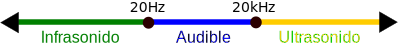
\includegraphics[scale=0.8]{desarrollo/rango_freq}
  \caption{Rango de frecuencias de sonido}
\end{figure}


Un oído sano y joven es capaz de detectar sonidos a partir de los 20
hercios. Los sonidos por debajo de esa frecuencia se conocen como
\textbf{infrasonidos}. Por otro lado, el límite auditivo en
frecuencias altas varía mucho con la edad: un adolescente puede oir
sonidos con frecuencias hasta los 18kHz, mientras que un adulto de
edad media solo suele llegar a captar sonidos de hasta 13kHz. El
límite genérico superior se establece en 20kHz, por encima de los
cuales los sonidos se denominan \textbf{ultrasonidos}.


\subsubsection{Amplitud}
La \textbf{amplitud} representa la energía que transporta la
onda. Cuando un instrumento u otro objeto genera una vibración, la
amplitud es la cantidad de movimiento que esa vibración genera.
Podría equipararse (de forma no estricta) a la intensidad del sonido:
cuanto mayor sea la amplitud, más fuerte se oirá el sonido.

\subsubsection{Fase}
Por último, la \textbf{fase} ($\varphi$) indica el desplazamiento
horizontal de la onda respecto del origen. Si la fase de una onda no
es cero, entonces parecerá que está \textit{desplazada} hacia la
derecha, si la fase es positiva, y hacia la izquierda si la fase es
negativa.
\begin{figure}[h]\centering
    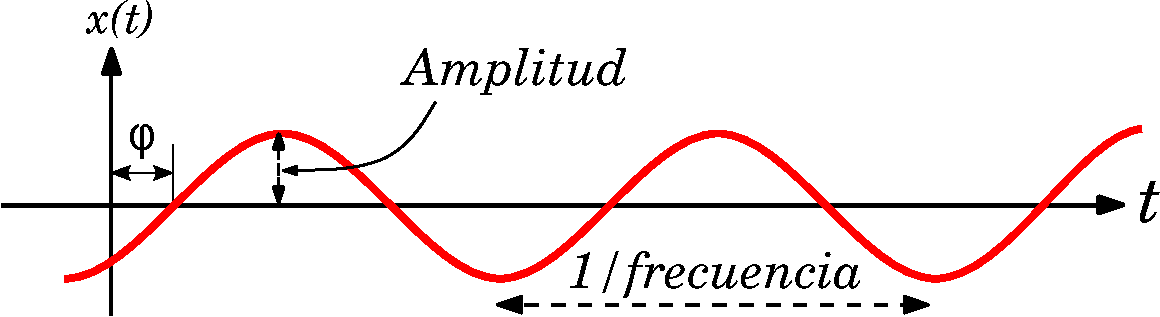
\includegraphics[scale=0.7]{desarrollo/onda}
    \caption{Componentes de una señal senoidal básica}
\end{figure}
\subsection{Descomposición de sonidos}
Para desarrollar oFlute nos interesa conocer la altura de la nota que
está tocando la flauta en un instante concreto. Para un tono puro,
podríamos conocer la altura fijándonos en su frecuencia. El problema
es que, en la naturaleza, \textbf{no existen} los tonos puros, sino
que los sonidos se componen de multitud de tonos de diferentes
amplitudes, frecuencias y fases. 

Afortunadamente, la teoría dicta que cualquier tono complejo puede
descomponerse como suma de tonos puros de distintas amplitudes, fases
y frecuencias, llamados \textbf{parciales}. La menor de todas las
frecuencias de los parciales se conoce como \textbf{frecuencia
  fundamental}, y es la que que dicta la altura general del sonido --
\textit{general}, ya que aunque el resto de frecuencias puede
corresponder a otras notas, es la altura de la frecuencia fundamental
la que mayor relevancia tiene en el sonido.

Un subconjunto de esos parciales, conocidos como \textbf{armónicos},
tienen frecuencias múltiplos de la frecuencia fundamental. Estos
armónicos sirven para enriquecer el sonido y, sobre todo, determinar
el \textbf{timbre musical} del origen del sonido: dos instrumentos (o
personas) pueden estar tocando la misma nota y emitir la misma
frecuencia fundamental, pero será el conjunto total de armónicos el
que nos ayude a distinguir qué instrumento está emitiendo el sonido.

Así pues, el objetivo es encontrar una forma de descomponer una señal
(el sonido) en sus componentes y analizar sus frecuencias, buscando la
frecuencia fundamental, que nos informará de la nota que se está tocando. 

\subsubsection{Representación gráfica de sonidos}

Las representación habitual de las señales se hace en el
\textbf{dominio del tiempo}, es decir, podemos observar cómo la señal
cambia a lo largo del tiempo, viendo el valor de su \textbf{amplitud}
en cada instante. Por otro lado, la representación en el
\textbf{dominio de la frecuencia} nos permite analizar una señal
respecto a las frecuencias que la componen, dividiendo la señal en sus
componentes.

En la figura \ref{fig:wavespectral} podemos comparar la representación de
un sonido en el dominio del tiempo, en \textbf{forma de ondas}, tal y
como aparecería en un osciloscopio, frente a su representación en
\textbf{forma espectral}, en la que el eje vertical indica la
frecuencia, y la intensidad del color indica la intensidad de esa
componente frecuencial en el sonido.

\begin{figure}[h!]
  \centering
  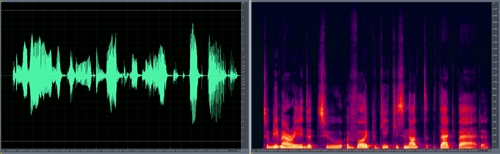
\includegraphics[scale=0.8]{desarrollo/wave_spectral}
  \caption{Forma de ondas vs representación espectral}
  \label{fig:wavespectral}
\end{figure}

\subsubsection{Herramientas de descomposición de señales}

La herramienta fundamental a la hora de descomponer una señal periódica, como
puede ser un sonido, en sus parciales o armónicos es el \textbf{análisis
  armónico} o \textbf{análisis de Fourier}. Esta rama del análisis matemático
estudia la representación de funciones o señales como superposición de ondas
básicas, y hoy en día se aplica en innumerables campos de la ciencia, desde el
procesamiento de señales para el reconocimiento de patrones, como es nuestro
caso, a la neurociencia.

Una de las herramientas más conocidas de este área es la \textbf{transformada de
  Fourier}. Se trata de una aplicación matemática que descompone una función en
su espectro de frecuencias a lo largo del dominio. Al aplicarla sobre una
función $f$, se define de la siguiente manera:

\[
g(\xi ) = \frac{1}{\sqrt{2\pi}} \int_{-\infty}^{+\infty} f(x)e^{-i\xi\,x} dx
\]

De cualquier modo, al estar tratando con un sistema digital como es una
computadora, no es viable aplicar esta definición de la transformada de Fourier,
ya que se basa en funciones continuas y derivables, y en nuestro caso
dispondremos de datos discretos.

De ahí, aparece la \textbf{transformada discreta de Fourier} o \textbf{DFT}, que
tiene el mismo uso que la transformada tradicional pero requiere que la función
de entrada sea una secuencia discreta y de duración finita.

Existe un gran número de aproximaciones al cálculo de la transformada de
Fourier, pero claramente el algoritmo más utilizado y eficiente es el
\textbf{FFT}, \textbf{Fast Fourier Transform}. A pesar de imponer algunas
limitaciones para mantener la eficiencia, el algoritmo FFT es la implementación
que más habitualmente se encuentra en los chips DSP. Por regla general, computar
la transformada de Fourier para $N$ puntos usando FFT tardaría un tiempo $O(N
\cdot log(N))$, mientras que hacerlo utilizando la definición estándar de la DFT
llevaría un tiempo $O(N^2)$.

A pesar de que fue el \textbf{DFT} el algoritmo que se utilizó finalmente en el
proyecto, se estudiaron otras posibles herramientas para la detección de la
frecuencia fundamental, como por ejemplo la \textbf{función de autocorelación},
que también suele utilizarse en análisis de señales para encontrar patrones
repetitivos, como señales enmascaradas por ruido. A pesar de ello, dada la poca
bibliografía encontrada sobre estas técnicas secundarias y la conocida
eficiencia de la transformada de Fourier, se decidió optar por la técnica más
conocida.

\subsection{Digitalización de sonidos}

Antes de poder aplicar ninguna técnica sobre los sonidos, es necesario
transformarlos de forma que el ordenador pueda trabajar con ellos.

\subsubsection{Captación de sonidos}
Lo más habitual a la hora de digitalizar un sonido es, primeramente, utilizar
algún dispositivo que transforme las ondas sonoras en algo que pueda
transmitirse al computador en forma de ondas eléctricas. Este dispositivo es el
\textbf{micrófono}, en nuestro caso de tipo \textbf{electret}, que es el más
utilizado en ordenadores personales, teléfonos móviles y demás dispositivos de
consumo con requisitos de audio de media o baja fidelidad.

Estos micrófonos constan de una membrana que vibra libremente cuando capta
cualquier onda acústica o de sonido, ya sea voz, música o ruidos, convirtiéndola
en una señal eléctrica de baja frecuencia y de muy poca tensión o voltaje,
semejante a la del sonido captado. Una vez que esta señal eléctrica llega a la
tarjeta de sonido, comienza la siguiente parte del proceso.

Curiosamente, el proceso es el inverso del que ocurre en un altavoz. Es por eso
que en el caso de algunos auriculares intrauditivos, como los que habitualmente
acompañan a los reproductores MP3 de bolsillo, es posible utilizarlos como
micrófonos de baja fidelidad. También es posible, aunque bastante más difícil,
utilizar ciertos micrófonos de escritorio como altavoces improvisados, limitados
a la reproducción de altas frecuencias.

\subsubsection{Muestreo de la señal}

El siguiente paso es el \textbf{muestreo} (o \textit{sampling}) de la señal. El
proceso consiste en medir la amplitud de la señal analógica en diferentes
puntos, uniformemente espaciados, a lo largo del tiempo. El número de veces que
se muestrea la señal por unidad de tiempo es conocido como \textbf{frecuencia de
  muestreo}, e influye directamente en la calidad de la digitalización del sonido.

La elección de la frecuencia de muestreo no suele ser trivial y tiene un impacto
importante en el rendimiento y calidad del sistema, ya que el número de
elementos a procesar es directamente proporcional a la frecuencia. 

Otro factor importante es la clase de sonidos que vamos a digitalizar. Por regla
general, los sonidos que se captan son los audibles por el oído humano. Tal y
como se comentó en la sección anterior, estos sonido son aquellos cuyas
frecuencias se encuentran por debajo de los 20 kHz. Existe un teorema dictado
por el ingeniero sueco \textbf{Harry Nyquist} que defiende que \textit{``la
  frecuencia de muestreo mínima requerida para muestrear una señal debe ser
  igual al doble de la máxima frecuencia contenida en la señal''}. En nuestro
caso, como la máxima frecuencia audible es de 20 kHz, lo normal será utiliar una
frecuencia de muestreo de 40 kHz. El estándar de CD, que normalmente se utiliza
como base de muestreo en la mayoría de tarjetas de sonido, amplía la tasa un
10\% con objeto de contemplar el uso de filtros no ideales, quedando la
frecuencia de muestreo en 44,1 kHz.

\subsubsection{Cuantificación de las muestras}

Una vez decidida la frecuencia de muestreo de la señal, será necesario acordar
qué utilizaremos para representar sus niveles de amplitud de forma digital. Este
proceso se conoce como \textbf{cuantificación}, y de él se desprenderá el número
de bits de cada muestra. Cabe notar que tanto el muestreo como la cuantificación
son procesos con \textbf{pérdidas}, ya que es imposible discretizar con total
fidelidad un rango continuo de tensiones.

Existen diferentes métodos para decidir los niveles a los que se ajustarán las
muestras. El más utilizado es el \textbf{PCM - modulación por impulsos
  codificados} en su variante \textit{uniforme}, que utiliza una escala uniforme
para digitalizar los valores de amplitud, a diferencia de la versión \textit{no
  uniforme}, que utiliza escalas como la logarítmica.

La \textbf{resolución de cuantificación} (o \textit{resolución digital}) más
habitual es de 16 bits, que es la utilizada en los CDs de audio. Esto nos
permite tener $2^{16} = 65536$ niveles distintos con los que cuantizar cada
muestra.

\subsubsection{Codificación de las muestras}

El último paso antes de tener los datos listos para el procesamiento es la
\textbf{codificación} en forma de bits. Aunque podría parecer un proceso trivial
-- convertir los valores digitales de las muestras en binario -- existen
multitud de parámetros que influyen a la hora de representar estas señales:
\begin{itemize}
\item \textbf{Tamaño de la muestra}: decidido en la cuantificación, la muestra
  puede tener tamaños desde los 8 a los 64 bits.
\item \textbf{Orden de los bytes}: para muestras de más de un byte, es
  importante decidir el orden de los mismos --
  \textbf{\textit{endianness}}. Popularmente, la mayoría de computadoras basadas
  en procesadores Intel utilizan \textit{little endian} -- esto es, se almacena
  primero los bytes de menos relevancia.
\item \textbf{Signo}: cualquier señal en forma de ondas pasa constantemente por
  el origen, de forma que la amplitud toma valores positivos y negativos a cada
  momento. Puede parecer intuitivo usar un entero con signo para la
  representación, pero también es posible utilizar uno sin signo, de forma que
  el origen se represente como la mitad del rango, ahorrándonos así posibles
  complicaciones en la representación de números negativos.
\item \textbf{Canales}: la mayoría de micrófonos de baja calidad producen sonido
  monoaural, de forma que solo es necesario utilizar un canal para su
  reproducción, a diferencia de los micrófonos estereofónicos que utilizan dos o
  más canales. En este aspecto, el flujo que se genera durante la digitalización
  de una señal estéreo es más complejo de procesar en tanto en cuanto los datos
  de cada canal vienen entrelazados en el flujo y, a veces, es difícil
  distinguirlos.
\end{itemize}

\section{Estudio del software disponible}

Existen algunas soluciones de software, juegos en la amplia mayoría de los
casos, que explotan la idea del análisis de sonido en tiempo real como principal
modo de interactuar con el usuario. En esta sección vamos a conocer algunas de
estas soluciones y las ideas que adquirimos de su estudio.

\subsection{Aplicaciones comerciales}

\subsubsection{SingStar}
\textbf{SingStar} fue el primer videojuego en explotar el uso de un micrófono
para que el usuario cantase y la aplicación reconociese el sonido. Apareció por
primera vez en mayo de 2004 para sistemas PlayStation 2, y desde entonces han
aparecido nada menos que 23 ediciones para este sistema y otras 6 para
PlayStation 3.

La ventaja de SingStar es la que da ser el primero en explotar una idea
atractiva, que rápidamente consiguió adeptos, principalmente entre el público
más joven. Este éxito se vio fortalecido por la firma de una gran cantidad de
contratos con discográficas a lo largo del tiempo, que permitió el lanzamiento
de ediciones regulares con los \textit{singles} más populares.

Las últimas ediciones de SingStar incluyen algoritmos avanzados que permiten,
entre otras opciones, añadir efectos a las voces de los usuarios ó
automáticamente limpiar las pista vocales de las canciones que los jugadores
carguen mediante almacenamiento externo.

\subsubsection{Lips}
\textbf{Lips} fue la respuesta de Microsoft a SingStar para sus sistemas
\textbf{Xbox 360}. El planteamiento es similar al de la versión de PlayStation,
aunque incluye una serie de mejoras bastante atractivas.

Los micrófonos utilizados en Lips son inalámbricos e incluyen un sistema de
detección de movimientos, de forma que es posible utilizarlos en secciones sin
pista vocal pero con percusión, siguiendo el ritmo a modo de maracas, o imitando
movimientos que aparecen en pantalla.

Desde el principio, Lips ha permitido utilizar canciones de terceros mediante la
conexión de un reproductor MP3. Esta opción solo estuvo disponible en sus
competidores después de la aparición de Lips. 

Además, Lips introdujo un sistema de juego colaborativo en forma de duetos, y
competitivo, en el que los jugadores cantaban secciones consecutivas de una
canción en busca de conseguir la mejor interpretación.

\subsubsection{Apariciones menores en otros títulos}
Aunque Lips y SingStar han sido los dos principales juegos del género, muchos
otros juegos musicales han incluido pequeñas pruebas y minijuegos que han hecho
uso de micrófonos. Por ejemplo, \textbf{DJ Hero}, \textbf{Guitar Hero },
\textbf{Band Hero} y \textbf{Def Jam Rapstar} permiten utilizar el micrófono
para añadir acompañamiento vocal al juego. La ventaja es que en la mayoría de
los casos, es posible utilizar los micrófonos de Lips y SingStar con estos
juegos de terceros, evitando tener que adquirir más dispositivos.

\subsection{Aplicaciones libres}

\subsubsection{UltraStar}
\textbf{UltraStar} fue el primer clon libre de SingStar. Fue desarrollado por
Patryk Cebula en 2007 y ha servido como base para diferentes forks
posteriores. El juego permite a varias personas jugar a la vez mediante la
conexión de varios micrófonos a una tarjeta de sonido, así como la adición de
nuevas canciones de forma sencilla mediante ficheros de configuración en formato
texto.

Aunque las versiones iniciales se liberaron bajo una licencia GNU GPL,
desgraciadamente en la actualidad UltraStar se encuentra con licencia
\textit{freeware}, utilizando como excusa inválida que así \textit{``[...] se
  protegen los datos privados de los usuarios al ser enviados al servidor
  mediante SSL''}. Realmente no existe razón para no utilizar software de código
abierto con SSL.

\subsubsection{UltraStar Deluxe}

\textbf{UltraStar Deluxe} nació como una modificación básica de UltraStar, pero
consiguió atraer la atención de muchos usuarios y desarrolladores, y finalmente
se constituyó como un producto indepèndiente. Los desarrolladores de UltraStar
Deluxe decidieron trabajar en varios aspectos que vieron mejorables respecto al
UltraStar original. Primero, mejorar la fiabilidad del programa, arreglando
numerosos bugs y aumentando el rendimiento. Segundo, trabajar la apariencia
visual, basándose en gran medida en los efectos del SingStar de PlayStation
3. Finalmente, facilitar la expansibilidad del sistema, permitiendo un gran
número de formatos para los ficheros de vídeo y audio, y creando un sistema de
scripting basado en Lua para los modos de juego colaborativos.

\subsubsection{Performous}

\textbf{Performous} es uno de los juegos musicales open source más
populares. Nació como una reescritura del UltraStar original, aunque
posteriormente lo superó con creces. La fortaleza de Performous reside en su
capacidad de reconocimento de voces, basado en la \textit{transformada rápida de
  Fourier (FFT)} y en una serie de algoritmos de post-procesamiento. 

Performous ha evolucionado con el tiempo, naciendo como un juego de cante pero
añadiendo características colectivas como Guitar Hero o Rock Band, permitiendo
el uso de controladores adicionales, como guitarras o baterías
electrónicas. Además, en las últimas versiones Performous incluye un modo de
baile, muy similar a los clásicos \textbf{DDR} o \textbf{StepMania}.

\section{Desarrollo con audio en GNU/Linux}

El desarrollo de aplicaciones que realicen tareas de sonido en sistemas
GNU/Linux es uno de los casos en los que más \textbf{dificultades} se
encuentran. Tradicionalmente, el soporte del hardware de sonido en estos
sistemas siempre ha sido de lo más básico, incluso limitándose, en ciertas
ocasiones, a la reproducción de sonido, ignorando por completo la
grabación. Afortunadamente, con el paso de los años el soporte ha ido mejorando
gracias a la colaboración de los fabricantes y a la proliferación del sonido
integrado en placa base.

A nivel de software, existen bastantes componentes diferentes, algunos
alternativos y otros complementarios entre sí, que pueden conducir a
confusiones. En otros sistemas operativos, como Windows o Mac OS, el programador
cuenta con una interfaz de sonido común, que se encarga de la mezcla y de la
comunicación de bajo nivel con la tarjeta de sonido. En GNU/Linux, dada su
naturaleza modular, esa misma tarea se descompone en diferentes sistemas, por lo
que una misma tarea puede realizarse de muchas formas distintas.

Buena muestra de ello es el artículo \textit{Welcome To The Jungle}
\footnote{\url{http://blogs.adobe.com/penguinswf/2007/05/welcome_to_the_jungle.html}},
en el que el desarrollador de Adobe, Mike Melanson, hace un repaso sobre la
\textit{jungla} que supone la programación de audio en Linux. El artículo es
antiguo y las cosas han mejorado desde entonces, pero aún así es muy fácil que
los no iniciados se sientan abrumados por la cantidad de opciones disponibles.

La organización de las capas de software se asemeja al siguiente diagrama.

\marginpar{PONER DIAGRAMA}

\subsection{Interfaces de bajo nivel, OSS y ALSA}
El elemento de menor nivel en esta \textit{escala} de componentes son las
interfaces de hardware, que podrían equipararse al \textit{driver de audio} de
Windows. En ambos casos se encuentran como módulos del kernel de Linux.

\subsubsection{OSS}
\textbf{Open Sound System} (OSS) fue durante muchos años la interfaz de audio
por defecto en todos los sistemas GNU/Linux. Está basada en el stándard UNIX
para la comunicación con dispositivos mediante las funciones POSIX habituales
(\texttt{open}, \texttt{read}, etc), lo que la hace relativamente sencilla de
utilizar.

Antiguamente, la mayor parte de los ordenadores personales con capacidades
multimedia utilizaban tarjetas de sonido basadas en la Creative Sound Blaster
16. De hecho, las tarjetas de la competencia incluían modos de emulación de esta
tarjeta. Su popularidad hizo que todos los esfuerzos en el desarrollo de audio
en Linux se concentraran en dar soporte a esta tarjeta, surgiendo unos drivers
de buena calidad. Finalmente, a la API generada se le dió el nombre de
\textit{Linux Sound API} y posteriormente, junto a los controladores de otras
tarjetas, se empaquetó en lo que hoy es conoce por OSS.

Por desgracia, los desarrolladores de OSS decidieron privatizar el
código. Aunque finalmente, en 2008, se volvió a liberar todo el código, para
entonces su mayor rival, ALSA, ya había tomado su lugar como API predeterminada
en el kernel de Linux.

\subsubsection{ALSA}
Como alternativa a OSS surgió \textbf{Advanced Linux Sound Architecture} (ALSA),
que acabó colocándose como la alternativa por defecto en todos los sistemas
GNU/Linux a partir de la versión 2.6 del kernel.

Entre sus características, ALSA permite la síntesis de sonidos MIDI mediante
hardware, soporte multiprocesador, configuración automática de tarjetas de
sonido, etcétera. En gran parte, los objetivos de ALSA fueron las deficiencias
de OSS en aquella época.

ALSA está estructurada en tres componente. La primera parte son los
controladores en el kernel. La segunda parte es una API para los
desarrolladores. Esta API es de muy bajo nivel, y es utilizada principalmente
por middlewares y frameworks en lugar de por aplicaciones de usuario. Por
último, el tercer componente es un mezclador que permite el multiplexado del
sonido.

Curiosamente, tanto ALSA como OSS han incluído una capa de emulación del otro
módulo, por lo que en un sistema con ALSA, los programas basados en OSS pueden
funcionar, aunque la calidad varíe enormemente de un caso a otro.

\subsection{Servidores de sonido}

Como se comentó previamente, uno de los problemas principales de OSS es que no
tenía mezclador, por lo que era imposible que varias aplicaciones emitieran
sonido a la vez. Para arreglar este problema surgieron los \textbf{servidores de
  sonido}. La principal tarea de estos servidores es la de gestionar el acceso a
los subsistemas de sonido, mezclando los flujos de sonido de las diferentes
aplicaciones en uno solo, de forma que sea posible escuchar el sonido de varios
programas al mismo tiempo.

Por otro lado, los servidores de sonido ofrecen una API más amigable, siendo más
sencillo programar a través de ellos. Aunque existen multitud de servidores de
sonido, los más conocidos son JACK y PulseAudio.

Aunque actualmente tanto ALSA como OSSv4 ofrece mezcla de audio, los servidores
de sonido siguen usándose por sus otras características, aunque varios autores
han declarado que en la mayoría de los casos son inútiles y solo empeoran el
rendimiento en general y la latencia en particular.

\subsubsection{JACK}

\textbf{JACK} es un servidor de sonido de uso profesional que proporciona
servicios de audio en tiempo real, consiguiendo latencias muy pequeñas. 

Su nombre (\textit{enchufe} en inglés) se debe a su arquitectura en forma de
conexiones, subtitulándose a menudo \textit{``Connection kit''}. Así, es posible
hacer conexiones de flujo de audio entre aplicaciones y la interfaz de audio de
igual forma que entre dos clientes, o con servidores de streaming online,
etcétera.

Hay gran cantidad de aplicaciones que ofrecen JACK como forma de comunicación de
audio, aunque su uso no está lo suficientemente extendido como para formar parte
por defecto de ninguna distribución mayoritaria.

\subsubsection{PulseAudio}
\textbf{PulseAudio} es otro servidor de sonido, multi-plataforma, que ha ganado
mucha popularidad en los últimos tiempos. Ofrece funcionalidades avanzadas, como
audio por red, control de volumen independiente por aplicación, ecualización del
sonido a nivel global, etcétera.

Se utiliza de forma oficial en muchas distribuciones, como Ubuntu o Fedora, e
incluso en dispositivos móviles de Nokia. Es de uso muy sencillo y se integra
fácilmente con muchos back-ends, tanto ALSA y OSS, ya comentados previamente,
como túneles RTP para la emisión por red.

PulseAudio permite también servir como reemplazo transparente de OSS, emulando
el acceso directo a los dispositivos (como \texttt{/dev/dsp}) mediante la
utilidad \texttt{padsp}. Además, existen muchas otras utilidades de línea de
comandos para controlar PulseAudio. Por ejemplo, \texttt{pacmd} nos permite
enviar comandos al demonio para 

PulseAudio fue la opción que finalmente se ha utilizado en este proyecto,
comentaremos los detalles más adelante.

\subsection{Otras APIs}

A los anteriores elementos, que en la mayoría de los casos son suficientes, hay
que sumarles una serie de APIs y frameworks independientes que, en mayor o menor
medida, han ido estableciéndose en distintos ámbitos: 

\begin{itemize}
\item \textbf{GStreamer} es un framework basado en GObject muy ligado al
  proyecto GNOME. Su funcionamiento se basa en complementos cuyas salidas y
  entradas es posible conectar, de modo que podemos comenzar con un módulo de
  lectura de ficheros, pasar a un decodificador, luego a un módulo de efectos y
  finalmente a la salida (o \textit{sink}). 

  La herramienta \texttt{gst-launch} permite probar el funcionamiento de estos
  módulos desde la línea de comandos. Por ejemplo, podemos hacer un
  \textit{loopback} (esto es, escuchar por los altavoces la entrada de audio,
  como el micrófono) mediante el siguiente comando:

\begin{verbatim}
gst-launch-0.10 alsasource ! alsasink
\end{verbatim}

\item \textbf{SDL Mixer} es una biblioteca que forma parte de SDL
  (\textit{Simple DirectMedia Layer}, un framework multimedia muy
  popular). Provee una API básica de reproducción de sonidos, y es muy utilizada
  en videojuegos por su facilidad de uso. El principal inconveniente es,
  precisamente, que su facilidad de uso se basa en un muy limitado rango de
  funciones. SDL Mixer no presenta ninguna capacidad de grabación o lectura de
  flujos de entrada, por lo que es imposible trabajar con micrófonos.

\item \textbf{RtAudio, PortAudio}. Ambas bibliotecas de entrada y salida de
  audio, escritas en C/C++, multi-plataforma pero con algunos
  fallos. Inicialmente, el proyecto se basó en RtAudio, pero se encontraron
  bastantes problemas con la biblioteca. A partir de ahí, se empezó a utilizar
  PortAudio, que funcionó bastante bien en las pruebas
  iniciales. Desafortunadamente, al comienzo del trabajo en el resto del
  proyecto se descubrieron problemas de estabilidad y finalmente se desechó.

\end{itemize}
